\documentclass[A4paper, 11pt]{article}

\usepackage[UTF8]{ctex}
\usepackage{amsfonts}
\usepackage{amsmath} 
\usepackage{amssymb}
\usepackage{array}
\usepackage{booktabs}
\usepackage{bm}
\usepackage{cite}
\usepackage{colortbl}
\usepackage{enumerate}
\usepackage{extarrows}
\usepackage{float}
\usepackage{geometry}
\usepackage{graphics}
\usepackage{graphicx}
\usepackage{ifthen}
\usepackage{listings}
\usepackage{longtable}
\usepackage{multicol}
\usepackage{pgf}
\usepackage{pgfplots}
\usepackage{pifont}
\usepackage{pstricks}
\usepackage{pst-node}
\usepackage{pst-tree}
\usepackage{pythonhighlight}
\usepackage{setspace}
\usepackage{tabularx}
\usepackage{tikz}
\usepackage{tocloft}
\usepackage{wrapfig}

\geometry{left=2cm, right=2cm, top=2cm, bottom=2cm}

\definecolor{emph}{RGB}{0,100,141}

\newcommand{\tabincell}[2]{\begin{tabular}{@{}#1@{}}#2\end{tabular}}
\newcommand*{\circled}[1]{\lower.7ex\hbox{\tikz\draw (0pt, 0pt) circle (.5em) node {\makebox[1em][c]{\small #1}};}}
\newcommand{\sfrac}[2]{\mbox{\small$\dfrac{#1}{#2}$}}
\renewcommand{\geq}{\geqslant}
\renewcommand{\leq}{\leqslant}
\renewcommand{\vec}{\overrightarrow}
\renewcommand{\d}{\,\mathrm{d}}
\newcommand{\lto}{\longrightarrow}
\newcommand{\ex}{\exists\,}
\newcommand{\R}{\mathbb{R}}
\newcommand{\<}{\,\langle\,}
\renewcommand{\>}{\,\rangle}
\newcommand{\normuv}[1]{\big|{#1}(u,v)\big|^2}
\newcommand{\infint}{\int_{-\infty}^{+\infty}}
\newcommand{\hollowstar}{\text{\ding{73}}}
\newcommand{\fullstar}{\text{\ding{72}}}

\newcommand{\Pro}[1]{\textbf{\large{Problem #1}} \vspace*{1ex}}
\newcommand{\Sol}{\textbf{\textit{Sol.}}}
\newcommand{\Ckp}{\textbf{\textit{Checkpoints}}}
\newcommand{\Pt}[1]{\textcolor{emph}{(#1 \ifthenelse{\equal{#1}{1}}{point}{points})}}

% Scalars
\renewcommand{\a}{\alpha}
% Matrices
\newcommand{\A}{\bm{A}}
\newcommand{\B}{\bm{B}}
\newcommand{\C}{\bm{C}}
\newcommand{\E}{\bm{E}}
% Vectors
\renewcommand{\b}{\bm{b}}
\newcommand{\x}{\bm{x}}
\newcommand{\y}{\bm{y}}
\newcommand{\z}{\bm{z}}
\renewcommand{\u}{\bm{u}}
\renewcommand{\v}{\bm{v}}
\newcommand{\w}{\bm{w}}
\newcommand{\0}{\mathbf{0}}
\newcommand{\1}{\mathbf{1}}
% Spaces
\newcommand{\V}{\mathcal{V}}
\newcommand{\X}{\mathcal{X}}
\newcommand{\Y}{\mathcal{Y}}
\newcommand{\F}{\mathcal{F}}
\newcommand{\N}{\mathcal{N}}
\renewcommand{\S}{\mathcal{S}}
% Names
\renewcommand{\sp}{\text{span}}
\newcommand{\rank}{\text{rank}}
\newcommand{\range}{\mathcal{R}}
\newcommand{\tr}{\text{tr}}

\newcommand{\typeset}{
    \setlength{\parindent}{0pt}
    \setlength{\parskip}{1ex}
    \setlength{\abovedisplayskip}{1ex}
    \setlength{\belowdisplayskip}{1ex}
}

\newcommand{\headbox}{
    \renewcommand{\arraystretch}{1.33}
    \begin{tabular}{|l|l|}
    \hline
    Name       & \hspace*{9em} \\
    \hline
    Student ID & \hspace*{9em} \\
    \hline
    \end{tabular} \hspace{131pt}
    \begin{tabular}{r}
        \textsc{CS\,270:\;Digital\;Image\;Processing} \\
        \textbf{\Large{Quiz 1}} \\
    \end{tabular}
    
    \vspace*{6ex}
    \renewcommand{\arraystretch}{1}
}

\begin{document}

\begin{spacing}{1.3}

\typeset

\textsc{\large{School\;of\;Information\;Science\;and\;Technology\\[2pt] ShanghaiTech\;University}}

\vspace*{5ex}

\textsc{\large{CS\,270:\;Digital\;Image\;Processing (Spring\;2024)}}

\vspace*{2.5ex} \textbf{\huge{Assignment 2}}

\vspace*{1.5ex} \textbf{\large{Due: 23:59, May 3, 2024}}

\vspace*{5ex}

\textbf{\large{Notes}}

\begin{itemize} \setlength{\parskip}{0.5ex} \vspace*{-1ex} 
    \item This assignment has \textbf{100 points} in total.
    \item Please prepare all your solutions in English.
    \item Please prepare your report with digital typesetting software (LaTeX, Microsoft Word, etc.). Handwritten reports, including digital handwriting on iPad etc., will not be accepted.
    \item Please submit your assignment to \textbf{Blackboard} as a \textbf{zip} file with its name formatted as\\ \texttt{DIP2024\_HW2\_ID\_ChineseName.zip}. The zip file should contain 3 things:
    \begin{enumerate}
        \item Your report named as \texttt{HW2\_Report\_ID\_Name.pdf};
        \item A folder named as \texttt{code} that stores your codes;
        \item A folder named as \texttt{images} that stores the original images in your report.
    \end{enumerate}
    For each problem, you should provide a separate code file that corresponds to it, with its name like \texttt{p3.m} (for Problem 3) or \texttt{p6a.m} (for Problem 6 (a)). Please make sure all paths in your codes are relative paths, so that we can run your codes and get your results without any modification.
\end{itemize}

\vspace*{2ex}
\textbf{\large{Policy on Plagiarism}}
\vspace*{1.5ex}

This is an individual homework. You can discuss the ideas and algorithms, but:
\begin{itemize} \setlength{\parskip}{0.5ex} \vspace*{-1.5ex}
    \item You cannot read, modify, and submit the codes of other students, nor allow other students to read, modify, and submit your codes.
    \item You cannot directly use generative AI tools to produce codes for submission. While you may consult generative AI for understanding the ideas and algorithms, the code you submit must be the result of your own individual understanding and efforts.
\end{itemize} \vspace*{-1.5ex}
We will utilize automated tools to check for plagiarism, and any violations will result in a zero score for this assignment and $20\%$ discount on total course grade.

\newpage

\begin{center}
    \textsc{I. Coding Part}
\end{center}

Please complete all the coding assignments using MATLAB. Make sure your results in the report are the same as the results of your codes. For general operations, the following functions may be useful:\\
\texttt{load}, \texttt{imread}, \texttt{double}, \texttt{im2double}, \texttt{uint8}, \texttt{imshow}, \texttt{zeros}, \texttt{size}, \texttt{montage}, \texttt{subplot}, \texttt{bar}.

\textcolor{red}{You must implement the core code in each question WITHOUT using relevant build-in functions.}\\


\vspace*{-3.75ex}
You can type \texttt{\textbf{help} FunctionName} in Command Window of MATLAB for detailed help text for the functionality specified by \texttt{FunctionName}.

\vspace*{6ex}

\Pro{1: Image sharpening}

(a) Apply the $3\times 3$ Sobel kernels ($x$-direction and $y$-direction) on \texttt{Figure 1.tif} to sharpen the image. Since the Sobel kernels are separable, you should implement this by the combination of simple kernels. Show the Sobel kernels and the corresponding processed images. (Implement your own \textbf{convolution} operator.) \Pt{10}

(b) Perform Gaussian Highpass filtering  $D_0=100$ on 'Figure 1.tif' in the frequency domain.  Show the Gaussian Highpass filter and the results (You can use fft2(), ifft2() and fftshift(), but not the built-in filtering function such as imfilter(), filter(), and filter2()). \Pt{15}

\begin{figure}[h]
        \centering
        \includegraphics[width=5.5cm]{figure/hw2/Figure1.jpg}
\end{figure}

\newpage

\Pro{2: Homomorphic filtering}

Implement Homomorphic filtering on 'PET-scan.tif' with the best paramters you think to improve the contrast of the subjet's limbs. Show the Homomorphic filter and filtered results. The preferable condition is that the variance of pixel values within the white box exceeds $3 \times 10^{-4}$, when the image is normalized to 0--1. \Pt{20}

\begin{figure}[h]
        \centering
        \includegraphics[width=5.5cm]{figure/hw2/PET-scan.jpg}
\end{figure}

\newpage

\Pro{3: Color Space Conversion}

Convert 'PeppersRGB.tif' from RGB to HSI color space, and then convert it back. Show the image in HSI space and the recovered result in RGB space (Hint: you need to normalize all channels to [0,1] in HSI space).\Pt{20}

\begin{figure}[h]
        \centering
        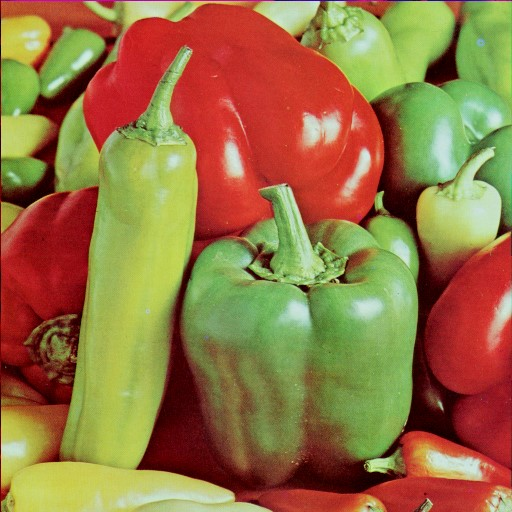
\includegraphics[width=5.5cm]{figure/hw2/PeppersRGB.jpg}
\end{figure}

\newpage


\Pro{4: Image Restoration}

In the process of image acquisition, the image blur caused by the relative movement between the acquisition device and target at the moment of exposure is called motion blur. In the spatial domain, the degenerate function model of motion blur can be expressed as:
\[
g(x, y) = h(x, y) \bigstar f(x, y) + n(x, y)
\]
Here, $g(x,y)$ represents the output image, $h(x,y)$ represents the degradation function, $f(x,y)$ represents the input image, and $n(x,y)$ represents the noise. The model in frequency domain can be expressed as:
\[
G(x, y) = H(x, y)F(x, y) + N(x, y)
\]
We can use \texttt{PSF= fspecial('motion',L,theta)} to simulate the convolution kernel $h(x, y)$. Here, \texttt{theta} refers to the angle between the direction of motion and the horizontal direction, which is called the direction of motion blur. $L$ refers to the distance the pixel moves in the direction of motion, which is called the motion blur distance.
\begin{figure}[h]
        \centering
        \includegraphics[width=5.5cm]{figure/hw2/blurred.jpg}
\end{figure}

Restore the \texttt{blurred.tif} following:

(a) Calculate the spectrum of the image, shift the zero frequency to the center of the spectrum. Display the spectrum logarithmically. You can use \texttt{fft2()}.\Pt{5}

(b) Estimate the parameters \texttt{L} and \texttt{theta} for \texttt{blurred.tif} (with a shape of \texttt{N} $\times$ \texttt{N}, \texttt{N} = 640).

Motion blur will produce periodic bright and dark stripes in the spectrogram. As shown in the example picture, \texttt{theta} is the angle between the stripe and the vertical direction, \texttt{d} represents the distance between two similar dark stripes (the distance between the two dark stripes near the center is \texttt{2d}), then \texttt{L=N/d}.

\begin{figure}[h]
        \centering
        \includegraphics[width=6.5cm]{figure/hw2/p5b.png}
\end{figure}

You can use the Radon transform to estimate the angle \texttt{theta}, and then rotate it 180-\texttt{theta} degree counterclockwise. Vertical projection of the rotated spectrogram can be used to estimate \texttt{L}, \texttt{L=N/d}.
Show the estimated parameters in your report. \Pt{15}

(c) Implement Wiener filtering with the estimated parameters, and choose the best K you think. You can obtain $H(u, v)$ through the \texttt{psf2otf()} function.  \Pt{15}





\end{spacing}

\end{document}